% Options for packages loaded elsewhere
\PassOptionsToPackage{unicode}{hyperref}
\PassOptionsToPackage{hyphens}{url}
%
\documentclass[
]{article}
\usepackage{amsmath,amssymb}
\usepackage{iftex}
\ifPDFTeX
  \usepackage[T1]{fontenc}
  \usepackage[utf8]{inputenc}
  \usepackage{textcomp} % provide euro and other symbols
\else % if luatex or xetex
  \usepackage{unicode-math} % this also loads fontspec
  \defaultfontfeatures{Scale=MatchLowercase}
  \defaultfontfeatures[\rmfamily]{Ligatures=TeX,Scale=1}
\fi
\usepackage{lmodern}
\ifPDFTeX\else
  % xetex/luatex font selection
\fi
% Use upquote if available, for straight quotes in verbatim environments
\IfFileExists{upquote.sty}{\usepackage{upquote}}{}
\IfFileExists{microtype.sty}{% use microtype if available
  \usepackage[]{microtype}
  \UseMicrotypeSet[protrusion]{basicmath} % disable protrusion for tt fonts
}{}
\makeatletter
\@ifundefined{KOMAClassName}{% if non-KOMA class
  \IfFileExists{parskip.sty}{%
    \usepackage{parskip}
  }{% else
    \setlength{\parindent}{0pt}
    \setlength{\parskip}{6pt plus 2pt minus 1pt}}
}{% if KOMA class
  \KOMAoptions{parskip=half}}
\makeatother
\usepackage{xcolor}
\usepackage[margin=1in]{geometry}
\usepackage{graphicx}
\makeatletter
\def\maxwidth{\ifdim\Gin@nat@width>\linewidth\linewidth\else\Gin@nat@width\fi}
\def\maxheight{\ifdim\Gin@nat@height>\textheight\textheight\else\Gin@nat@height\fi}
\makeatother
% Scale images if necessary, so that they will not overflow the page
% margins by default, and it is still possible to overwrite the defaults
% using explicit options in \includegraphics[width, height, ...]{}
\setkeys{Gin}{width=\maxwidth,height=\maxheight,keepaspectratio}
% Set default figure placement to htbp
\makeatletter
\def\fps@figure{htbp}
\makeatother
\setlength{\emergencystretch}{3em} % prevent overfull lines
\providecommand{\tightlist}{%
  \setlength{\itemsep}{0pt}\setlength{\parskip}{0pt}}
\setcounter{secnumdepth}{-\maxdimen} % remove section numbering

%\newcommand{\beginsupplement}{%
%        \setcounter{table}{0}
%        \renewcommand{\thetable}{\arabic{table}}%
%        \setcounter{figure}{0}
%        \renewcommand{\thefigure}{\arabic{figure}}%
%     }

\newcommand{\beginsupplement}{
	\renewcommand{\figurename}{Supplementary Figure}
	\setcounter{figure}{0}
}

%\usepackage{xr}
%\externaldocument{Supplementary_File1}

\usepackage{lineno}
\linenumbers

\usepackage[compress, super]{natbib}

\usepackage{setspace} \doublespacing

\usepackage{siunitx}

\usepackage[utf8]{inputenc}
\usepackage{amsmath}
\usepackage{algorithm}
\usepackage{algpseudocode}

\algrenewcommand\algorithmicrequire{\textbf{Input:}}
\algrenewcommand\algorithmicensure{\textbf{Output:}}
\ifLuaTeX
  \usepackage{selnolig}  % disable illegal ligatures
\fi
\IfFileExists{bookmark.sty}{\usepackage{bookmark}}{\usepackage{hyperref}}
\IfFileExists{xurl.sty}{\usepackage{xurl}}{} % add URL line breaks if available
\urlstyle{same}
\hypersetup{
  pdftitle={Supplemental File for: Transcripts with high distal heritability mediate genetic effects on complex metabolic traits},
  hidelinks,
  pdfcreator={LaTeX via pandoc}}

\title{Supplemental File for: Transcripts with high distal heritability
mediate genetic effects on complex metabolic traits}
\author{}
\date{\vspace{-2.5em}}

\begin{document}
\maketitle

\beginsupplement

\subsection{Supplementary Figures}\label{supplementary-figures}

\begin{figure}[ht!]
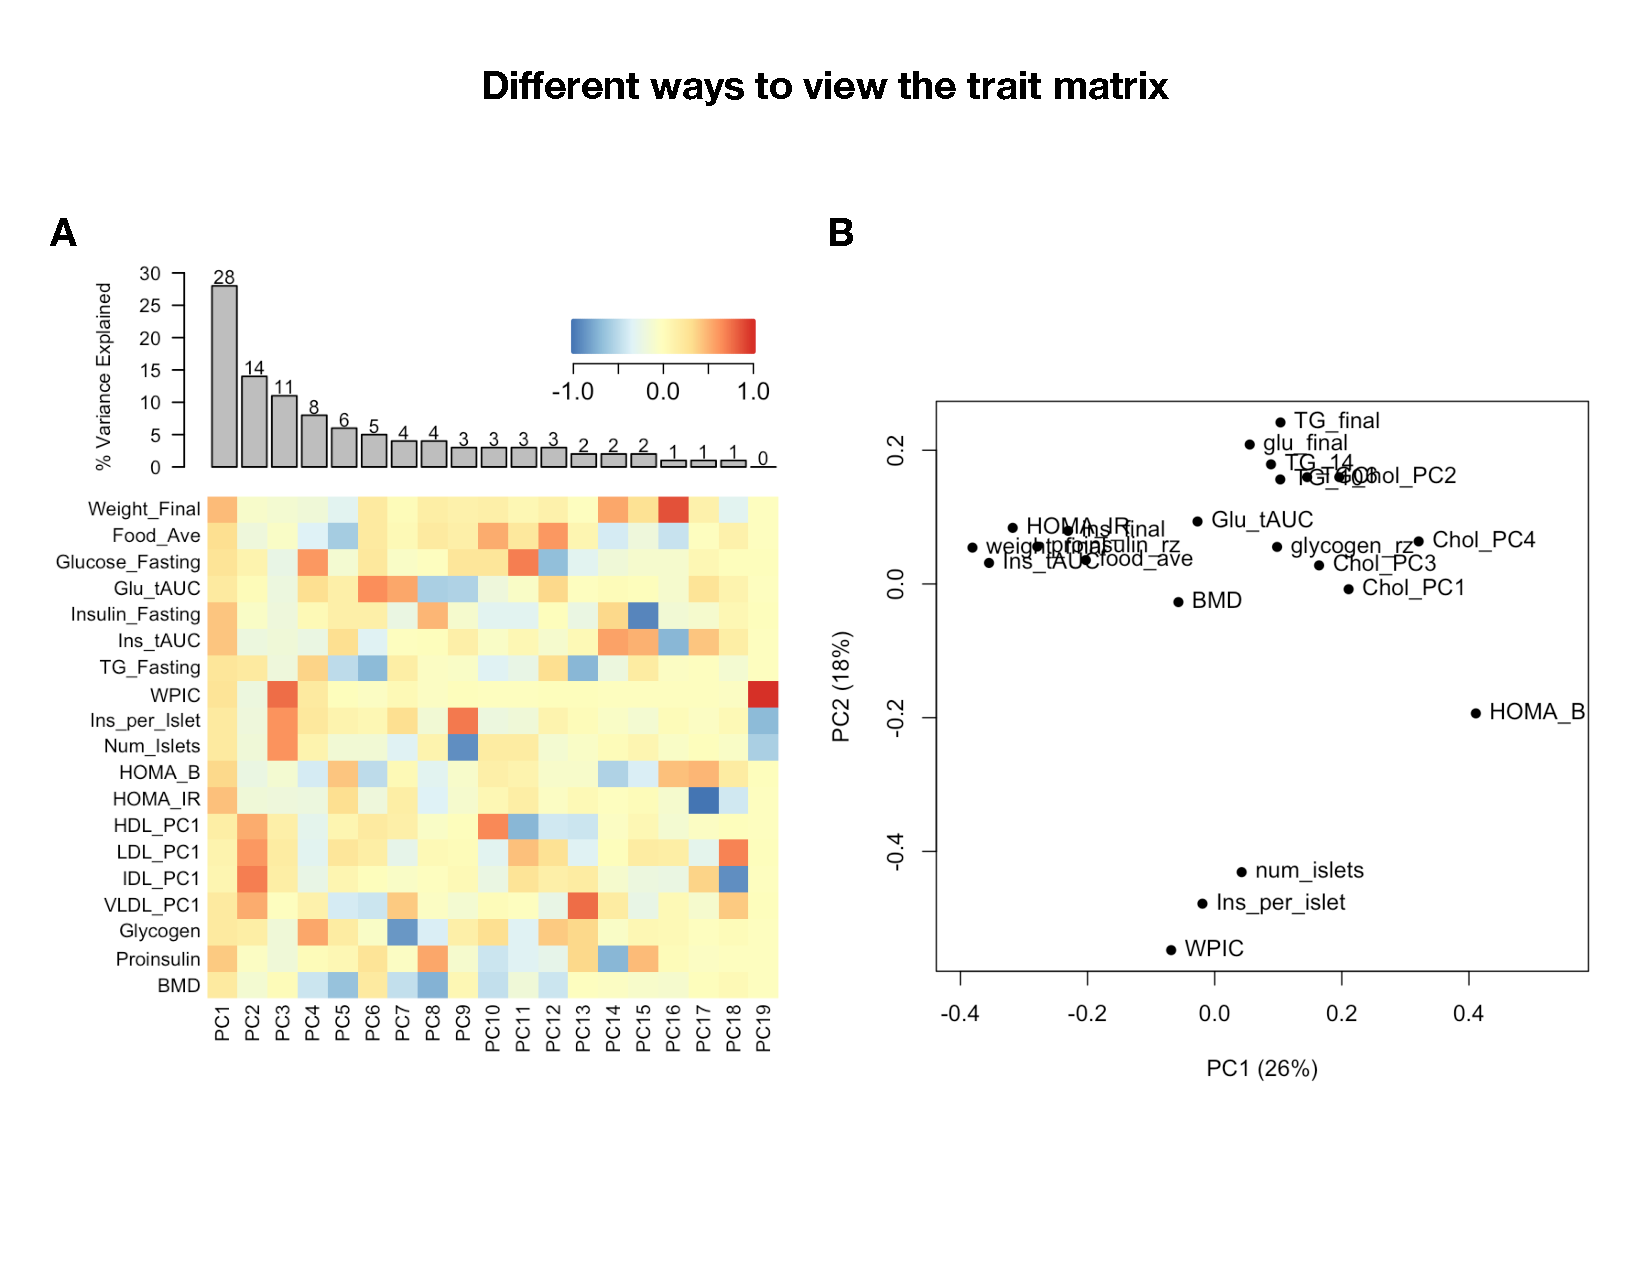
\includegraphics[width=\textwidth]{Figures/Supp_Fig_Trait_Decomposition.pdf} 
\caption{Trait matrix decomposition. \textbf{A} The heat map 
shows the loadings of each trait onto each principal component 
of the trait matrix. The bars at the top show the percent variance 
explained for each principal component. \textbf{B} Traits plotted 
by the first and second principal components of the trait matrix. 
This view shows clustering of traits into insulin- and 
weight-related traits, lipid-related traits, and ex-vivo 
pancreatic measurements.
}
\label{fig:trait_decomp}
\end{figure}

\begin{figure}[ht!]
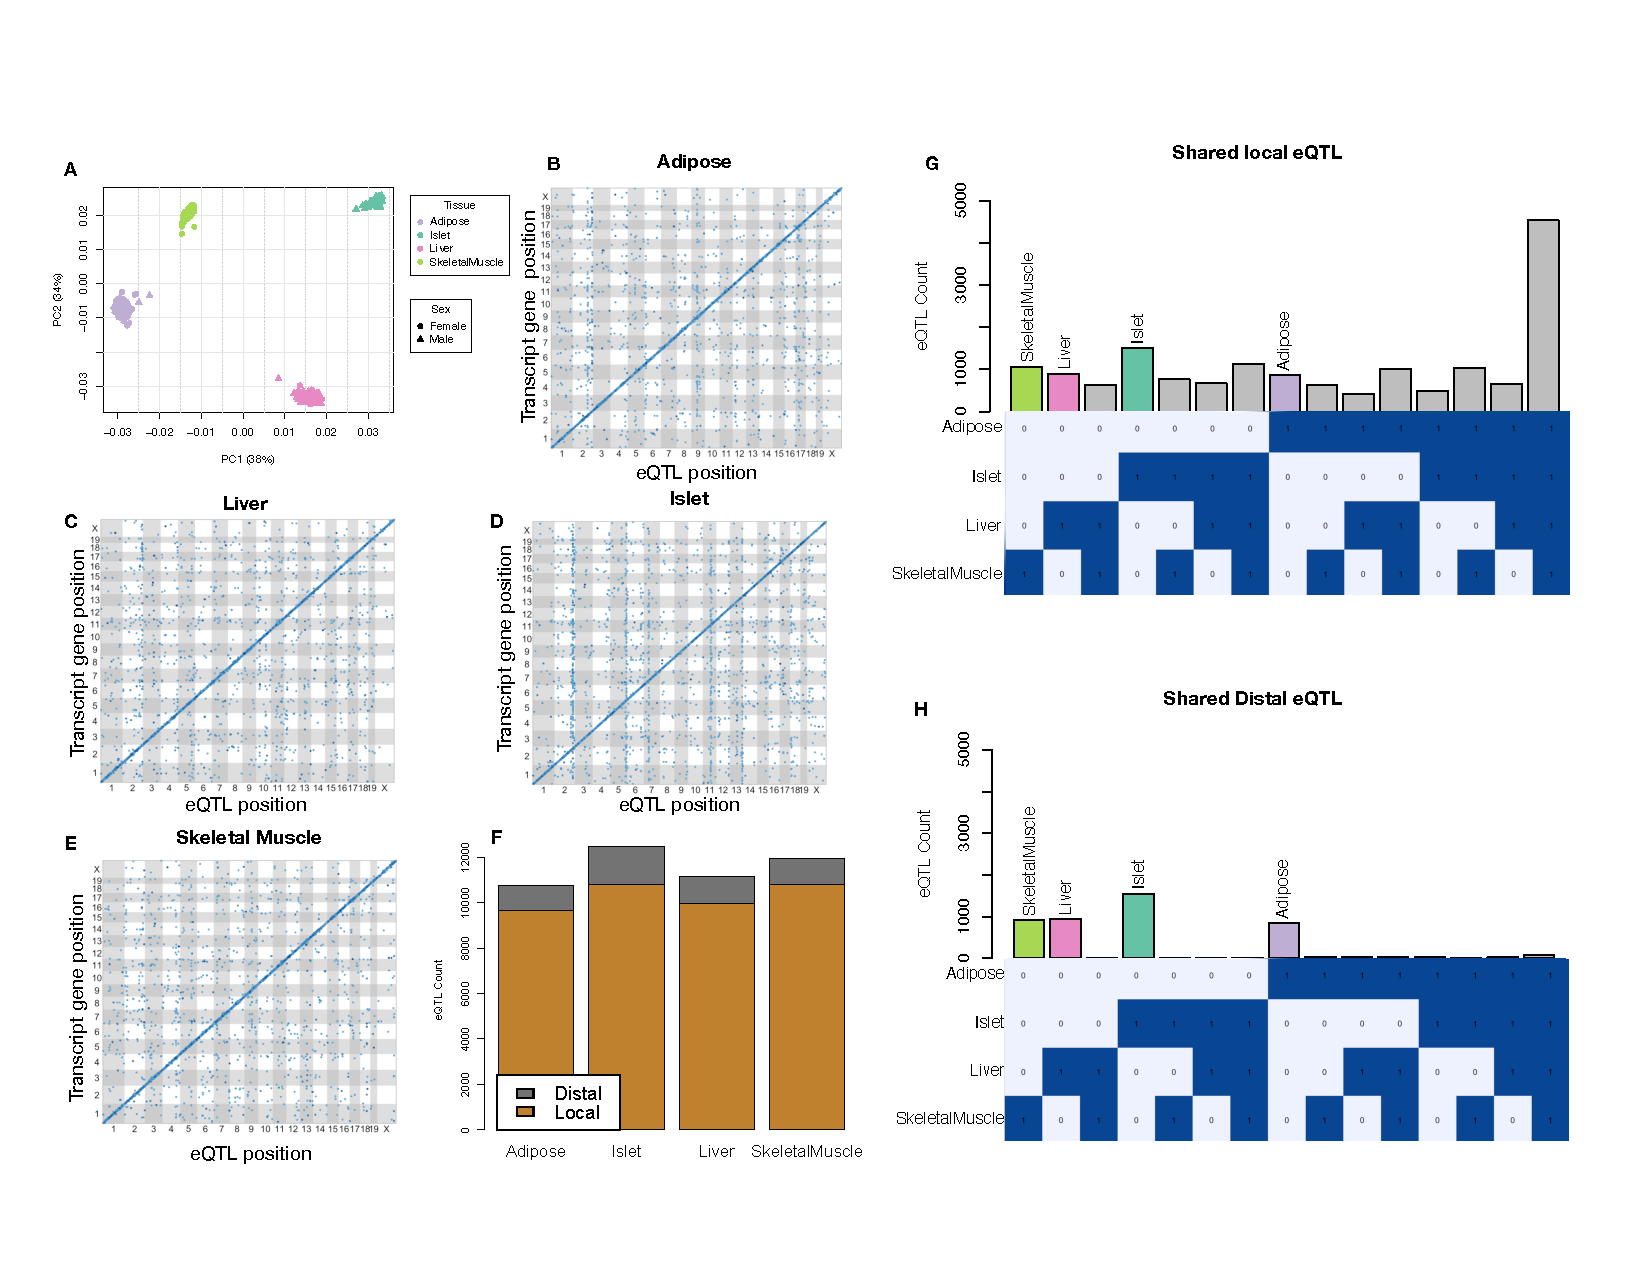
\includegraphics[width=\textwidth]{Figures/Supp_Fig_eQTL.pdf} 
\caption{Overview of eQTL analysis in DO mice. \textbf{A.} RNA seq 
samples from the four different tissues clustered by tissue. 
\textbf{B.-E.} eQTL maps are shown for each tissue. The $x$-axis 
shows the position of the mapped eQTL, and the $y$-axis shows the 
physical position of the gene encoding each mapped transcript. 
Each dot represents an eQTL with a minimum LOD score of 8, which 
represents a genome-wide permutation-based threshold of p < 0.01. The 
dots on the diagonal are locally regulated eQTL for which the mapped 
eQTL is at the within 4Mb of the encoding gene. Dots off the diagonal 
are distally regulated eQTL for which the mapped eQTL is distant from 
the gene encoding the transcript. \textbf{F.} Comparison of the total 
number of local and distal eQTL with a minimum LOD score of 8 in each 
tissue. All tissues have comparable numbers of eQTL. Local eQTLs are 
much more numerous than distal eQTL. \textbf{G.} Counts of transcripts 
with local eQTL shared across multiple tissues. The majority of local 
eQTLs were shared across all four tissues. \textbf{H.} Counts of 
transcripts with distal eQTL shared across multiple tissues. The majority 
of distal eQTL were tissue-specific and not shared across multiple tissues. 
For both G and H, eQTL for a given transcript were considered shared in two 
tissues if they were within 4Mb of each other. Colored bars indicate the 
counts for individual tissues for easy of visualization.
}
\label{fig:eQTL}
\end{figure}

\begin{figure}[ht!]
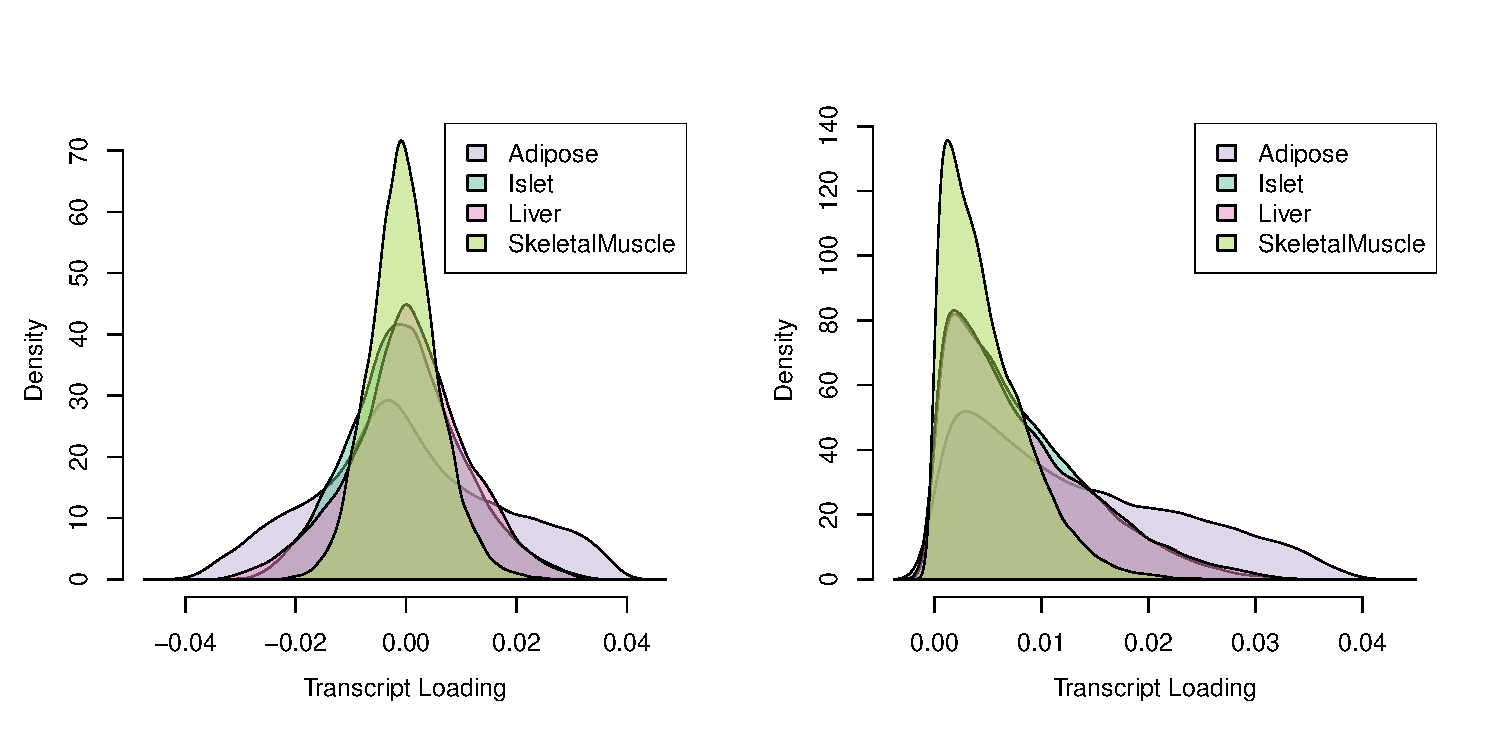
\includegraphics[width=\textwidth]{Figures/Supp_Fig_transcript_load_comparison.pdf} 
\caption{Direct comparisons of transcript loadings across tissues. \textbf{A.}
Distributions of transcript loadings are shown as density curves and are 
differentially colored to indicate tissue. Transcripts in adipose tissue had 
both the largest positive and negative loadings. \textbf{B.} Direct comparison
of absolute values of transcript loadings across tissues. Transcripts in adipose
tissue had the largest loadings overall, while those in skeletal muscle had the
smallest.
}
\label{fig:transcript_loading_comparison}
\end{figure}

\begin{figure}[ht!]
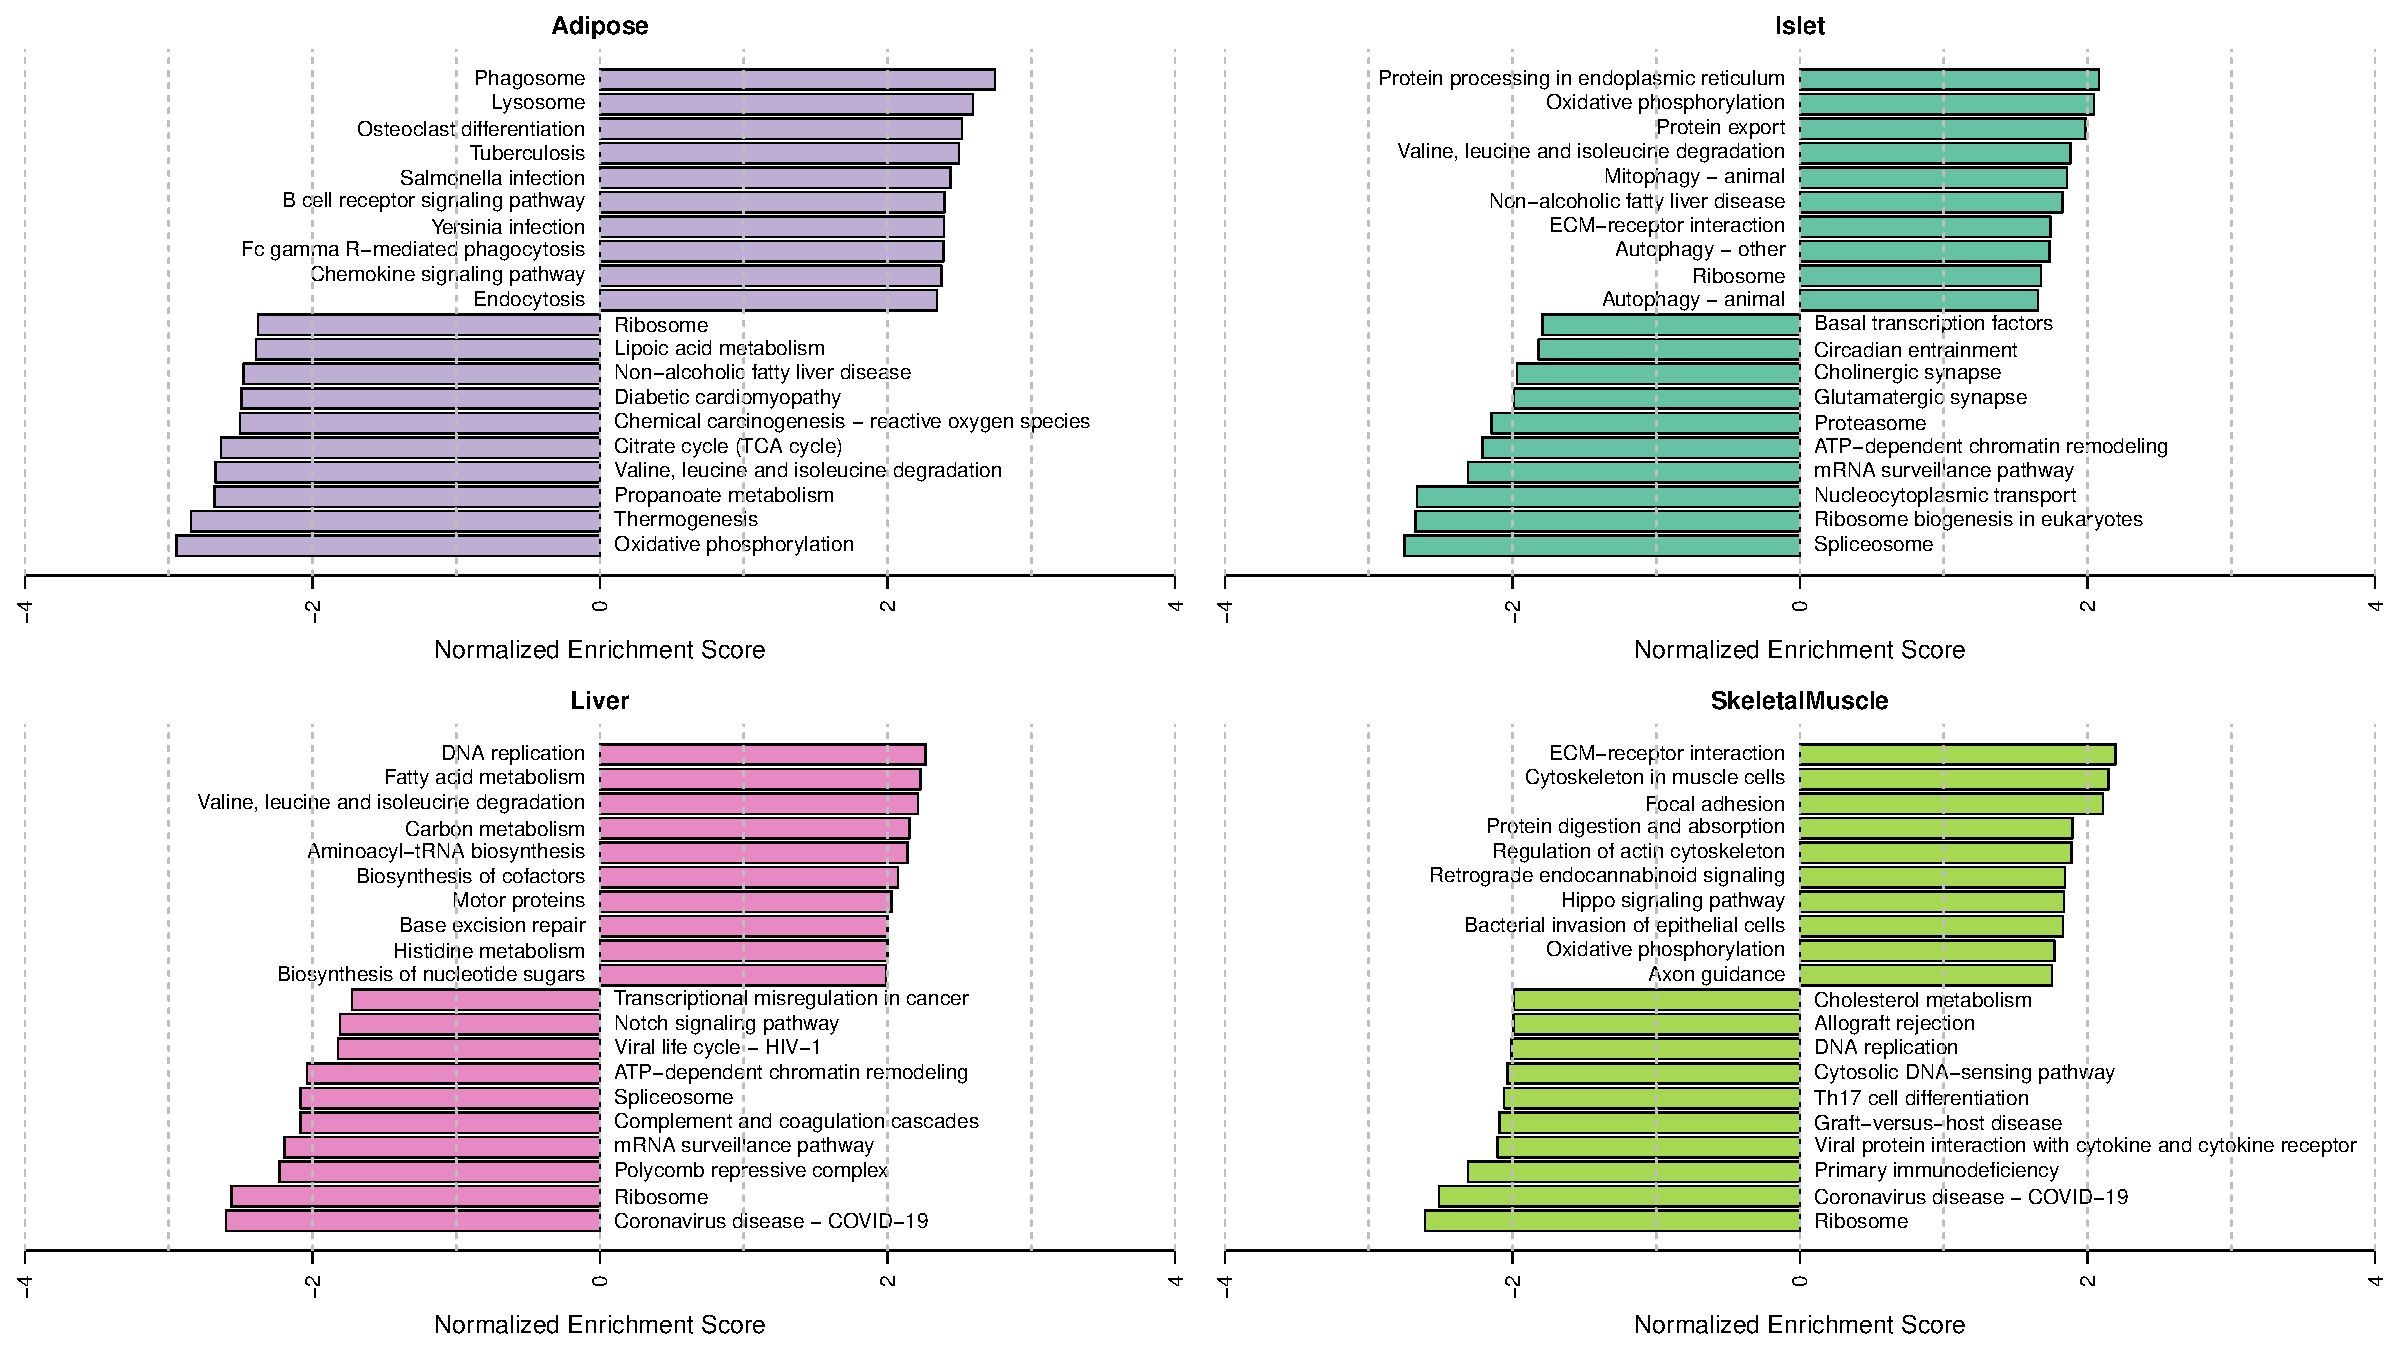
\includegraphics[width=\textwidth]{Figures/Supp_Fig_enrichments_KEGG.pdf} 
\caption{Bar plots showing normalized enrichment scores (NES) for KEGG 
pathways as determined by fast gene score enrichment analysis (fgsea). 
Only the top 10 positive and top 10 negative scores are shown. Colors 
indicate tissue. The name beside each bar shows the name of each enriched 
KEGG pathway.
}
\label{fig:top_enrich_kegg}
\end{figure}

\begin{figure}[ht!]
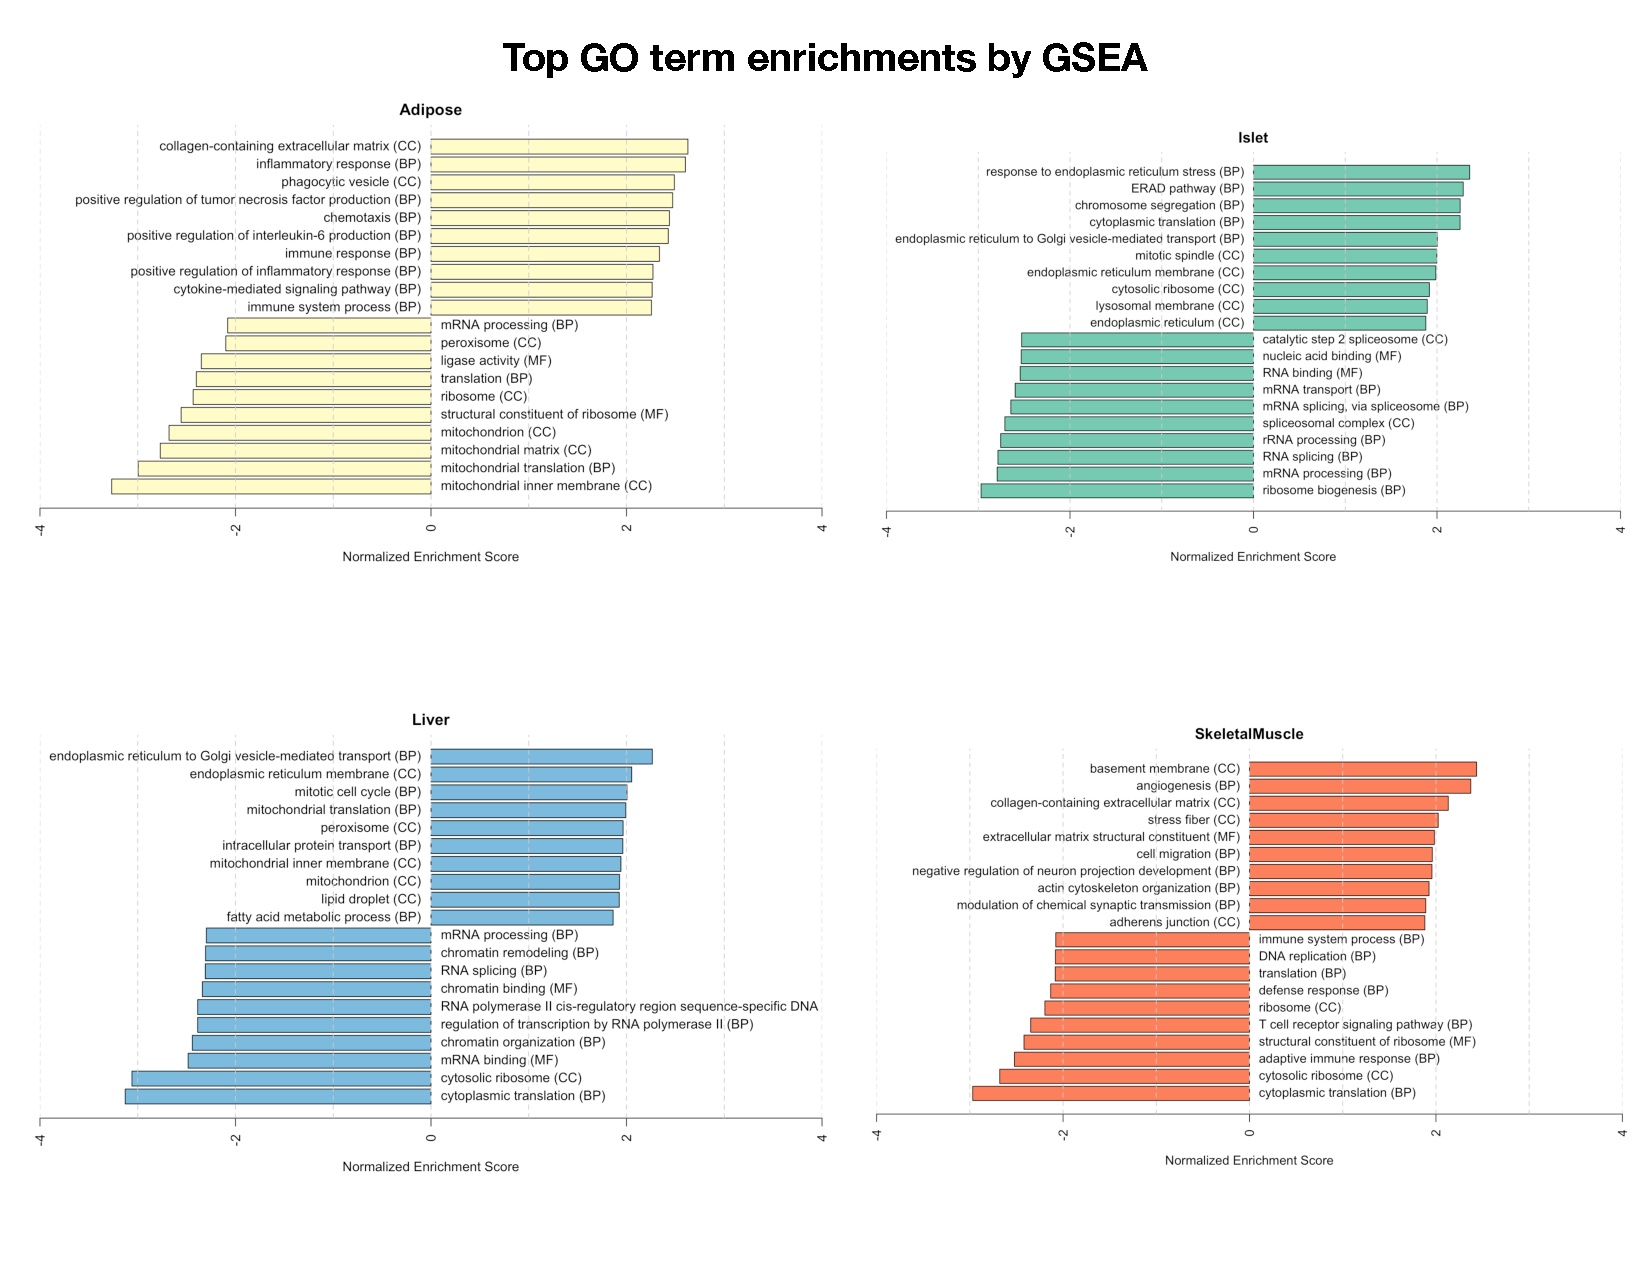
\includegraphics[width=\textwidth]{Figures/Supp_Fig_enrichments_GO.pdf} 
\caption{Bar plots showing normalized enrichment scores (NES) for GO 
terms as determined by fast gene score enrichment analysis (fgsea). 
Only the top 10 positive and top 10 negative scores are shown. Colors 
indicate tissue. The name beside each bar shows the name of each enriched 
GO term. The letters in parentheses indicate whether the term is from the 
biological process ontology (BP), the molecular function ontology (MF), 
or the cellular compartment ontology (CC).
}
\label{fig:top_enrich_go}
\end{figure}

\begin{figure}[ht!]
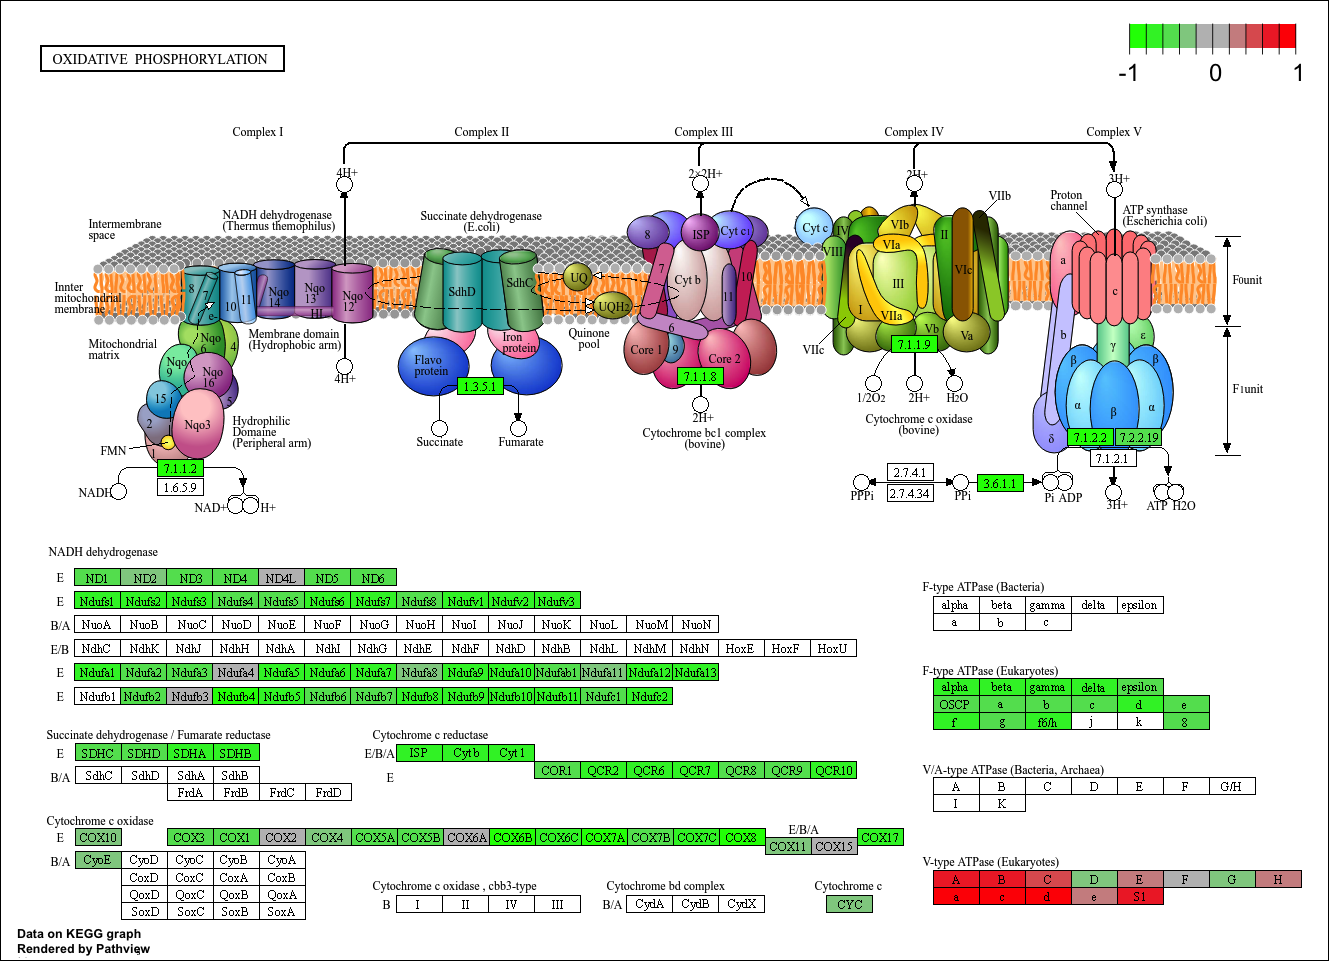
\includegraphics[width=\textwidth]{Figures/Supp_Fig_OxPhos.png} 
\caption{The KEGG pathway for oxidative phosphorylation in 
mice. Each element is colored based on its HDMA loading from adipose
tissue scaled to run from -1 to 1. Genes highlighted in green had 
negative loadings, and those highlighted in red had positive loadings. 
Almost the entire pathway was strongly negatively loaded indicating 
that increased expression of genes involved in oxidative phosphorylation
was associated with reduced MDI.
}
\label{fig:oxPhos}
\end{figure}

\begin{figure}[ht!]
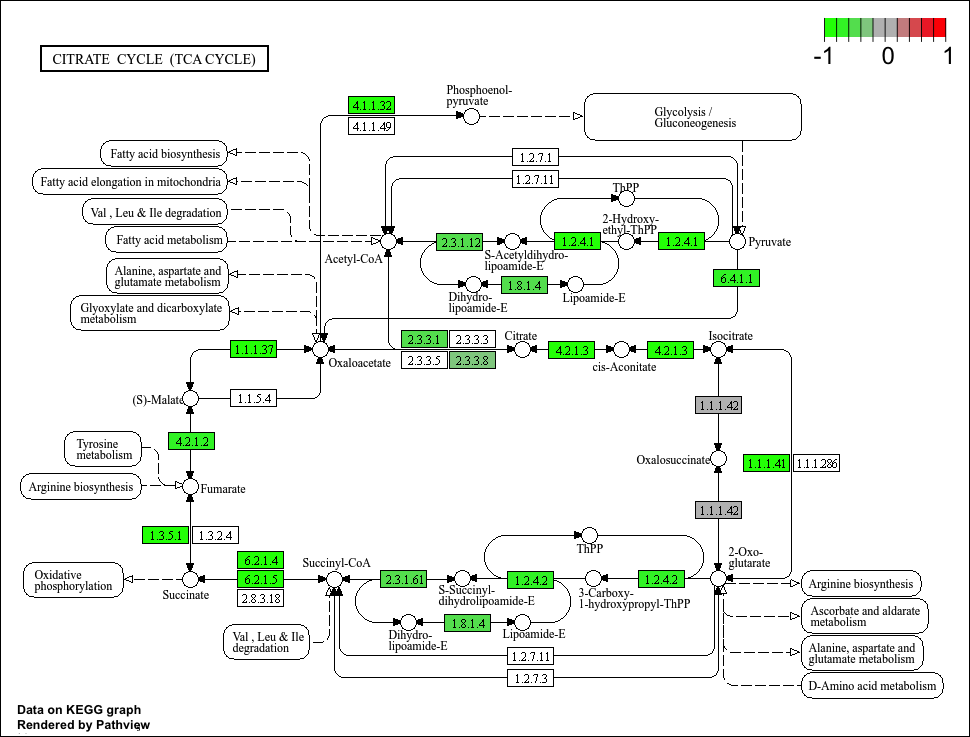
\includegraphics[width=\textwidth]{Figures/Supp_Fig_TCA.png} 
\caption{The KEGG pathway for the TCA (citric acid) cycle in 
mice. Each element is colored based on its HDMA loading from adipose
tissue scaled to run from -1 to 1. Genes highlighted in green had 
negative loadings, and those highlighted in red had positive loadings. 
Many genes in the cycle were strongly negatively loaded indicating 
that increased expression of genes involved in the TCA cycle was 
associated with reduced MDI.
}
\label{fig:TCA_cycle}
\end{figure}

\begin{figure}[ht!]
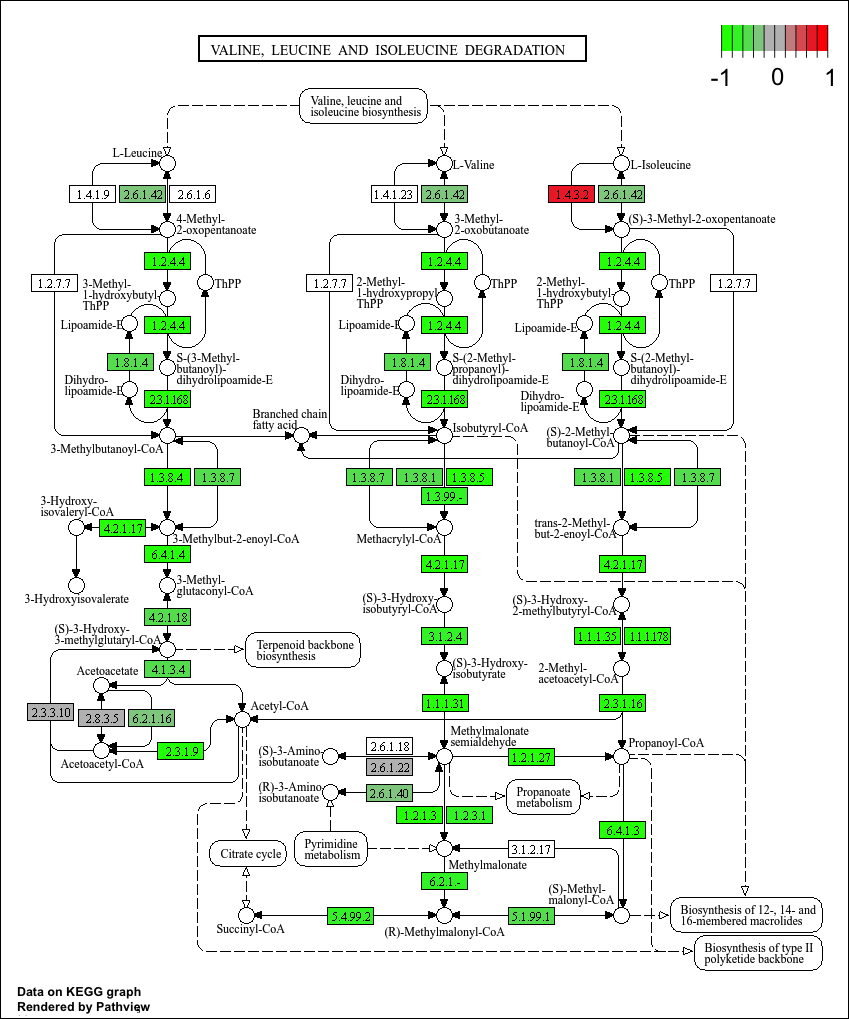
\includegraphics[width=\textwidth]{Figures/Supp_Fig_Branched_Chain.png} 
\caption{The KEGG pathway for branched-chain amino acid degradation in 
mice. Each element is colored based on its HDMA loading from adipose
tissue scaled to run from -1 to 1. Genes highlighted in green had 
negative loadings, and those highlighted in red had positive loadings. 
Almost the entire pathway was strongly negatively loaded indicating 
that increased expression of genes involved in branched-chain amino acid 
degradation was associated with reduced MDI.
}
\label{fig:bcaa_degrataion}
\end{figure}

\begin{figure}[ht!]
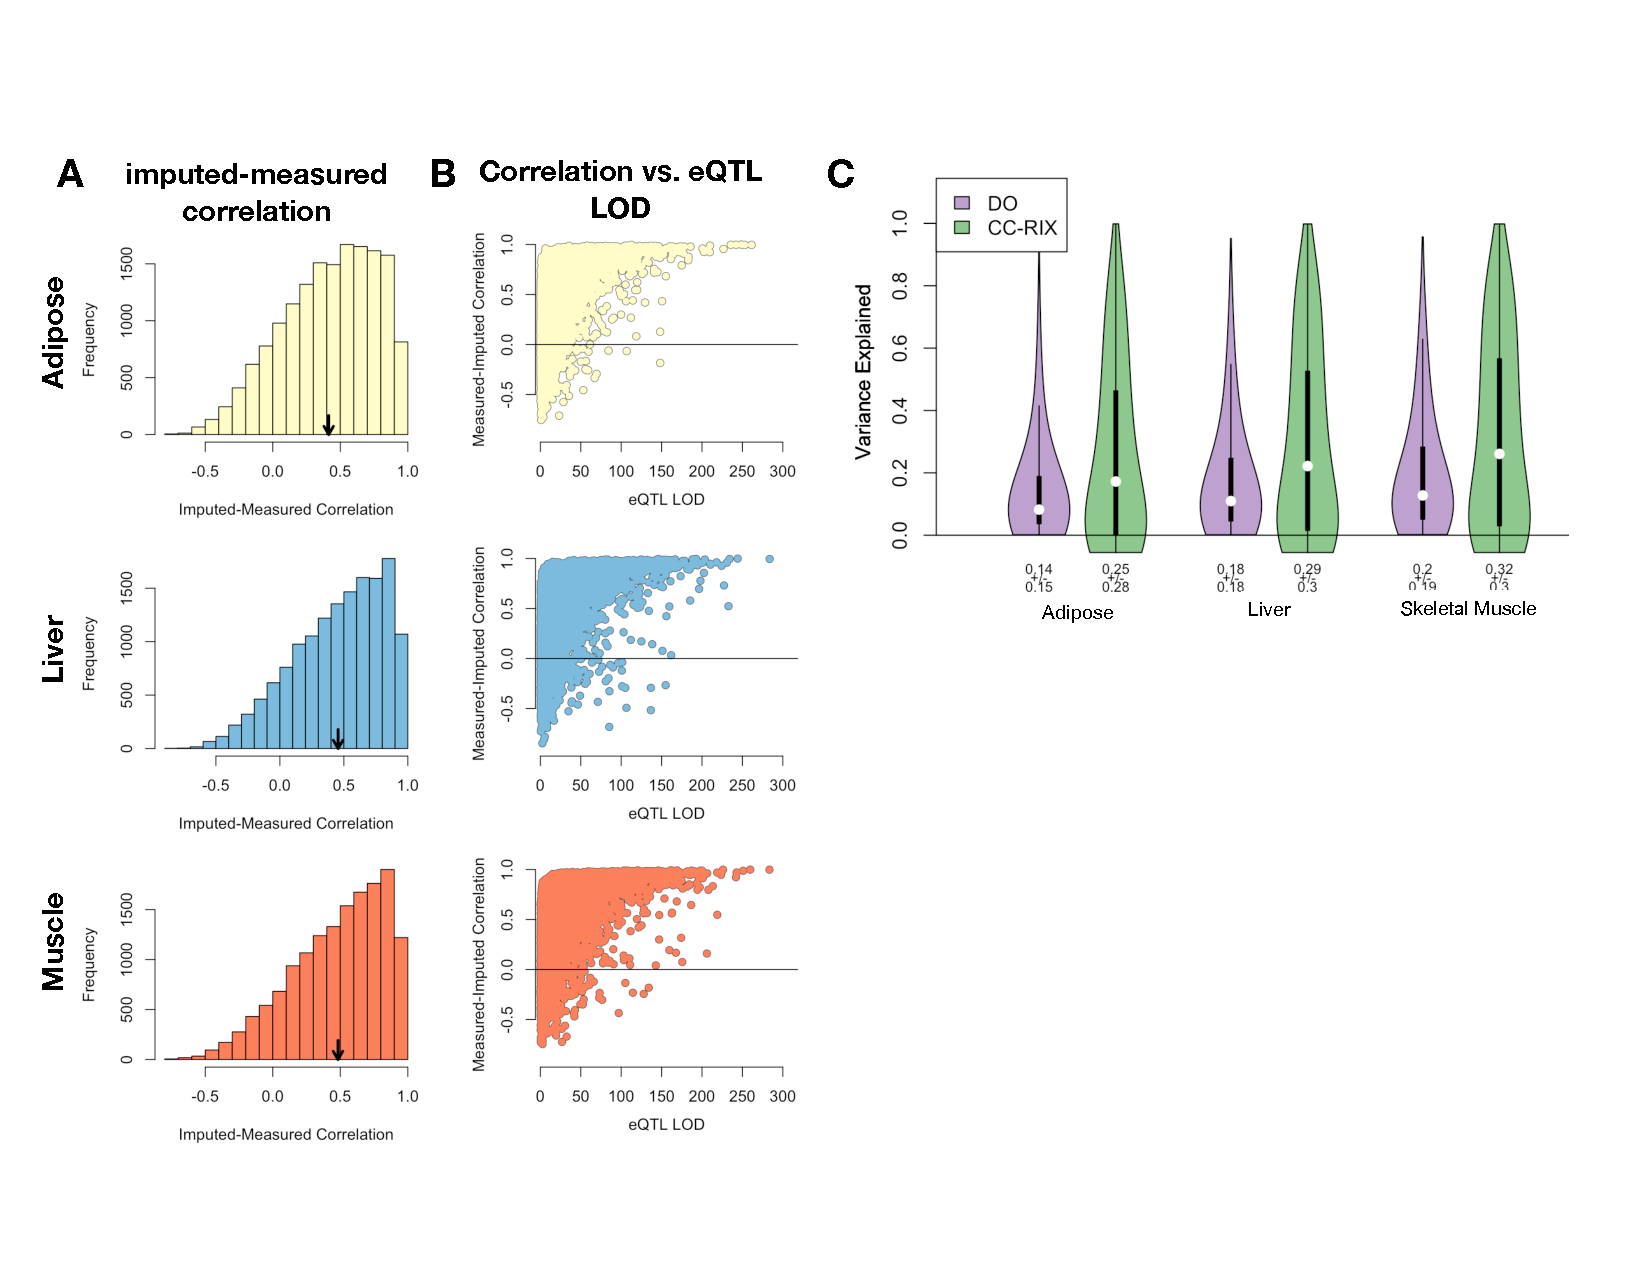
\includegraphics[width=\textwidth]{Figures/Supp_Fig_CC-RIX_Imputation.pdf} 
\caption{Validation of transcript imputation in the CC-RIX. \textbf{A.} 
Distributions of correlations between imputed and measured transcripts 
in the CC-RIX. The mean of each distribution is shown by the red line. 
All distributions were skewed toward positive correlations and had
 positive means near a Pearson correlation (r) of 0.5. \textbf{B.} 
 The relationship between the correlation between measured and 
 imputed expression in the CC-RIX (x-axis) and eQTL LOD score. As 
 expected, imputations are more accurate for transcripts with strong 
 local eQTLs. \textbf{C.} Distributions of variance explained by local 
 genotype across all transcripts in the DO and CC-RIX. 
}
\label{fig:cc_imputation}
\end{figure}

\begin{figure}[ht!]
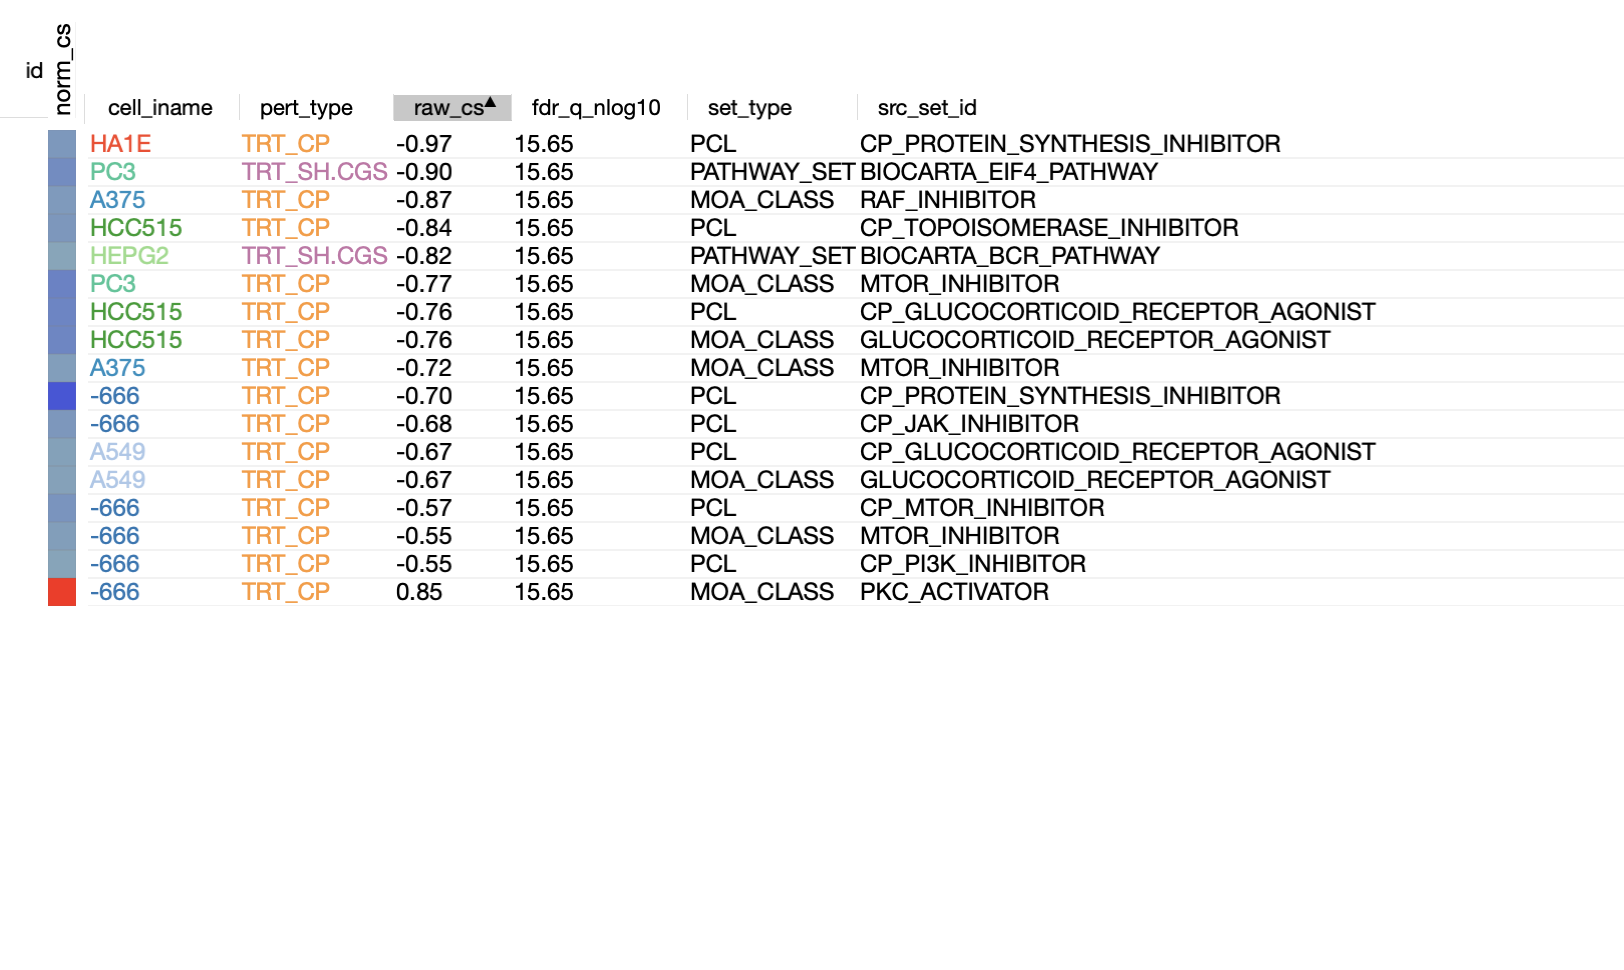
\includegraphics[width=\textwidth]{Figures/Supp_Fig_Adipose_all_cell_types.png} 
\caption{CMAP results using the \textit{adipose} tissue composite transcript as 
an input. Table includes results from \textit{all cell types} sorted with a 
$-log_{10}(q) > 15$. The results are sorted by the correlation of the 
query to the input with the most negative results at the top.
}
\label{fig:clue_adipose_all}
\end{figure}

\begin{figure}[ht!]
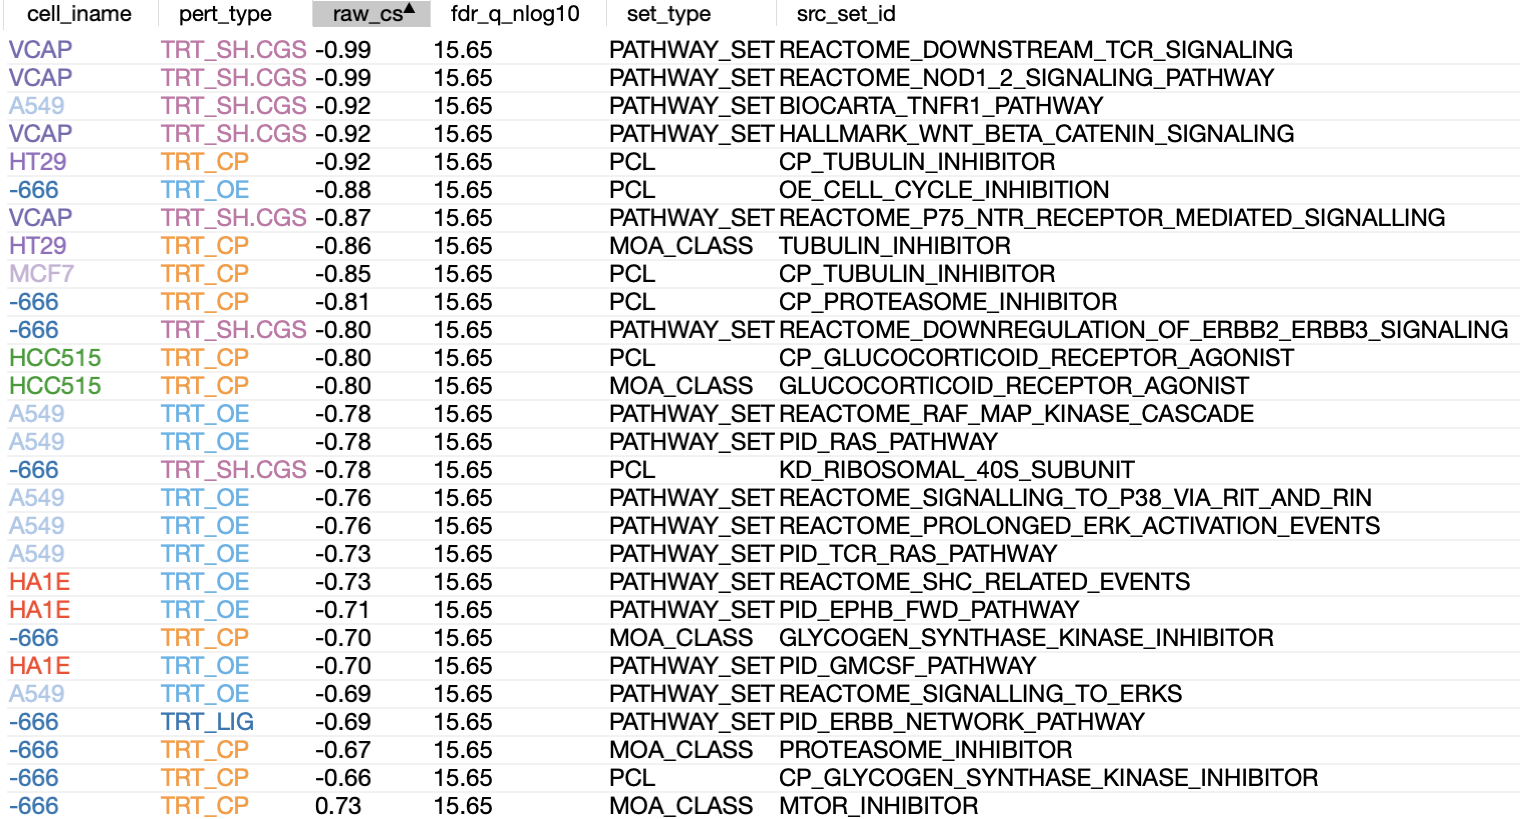
\includegraphics[width=\textwidth]{Figures/Supp_Fig_Islet_all_cell_types.png} 
\caption{CMAP results using the \textit{pancreatic islet} tissue composite transcript 
as an input. Table includes results from \textit{all cell types} sorted with a 
$-log_{10}(q) > 15$. The results are sorted by the correlation of the 
query to the input with the most negative results at the top.
}
\label{fig:clue_islet_all}
\end{figure}

\begin{figure}[ht!]
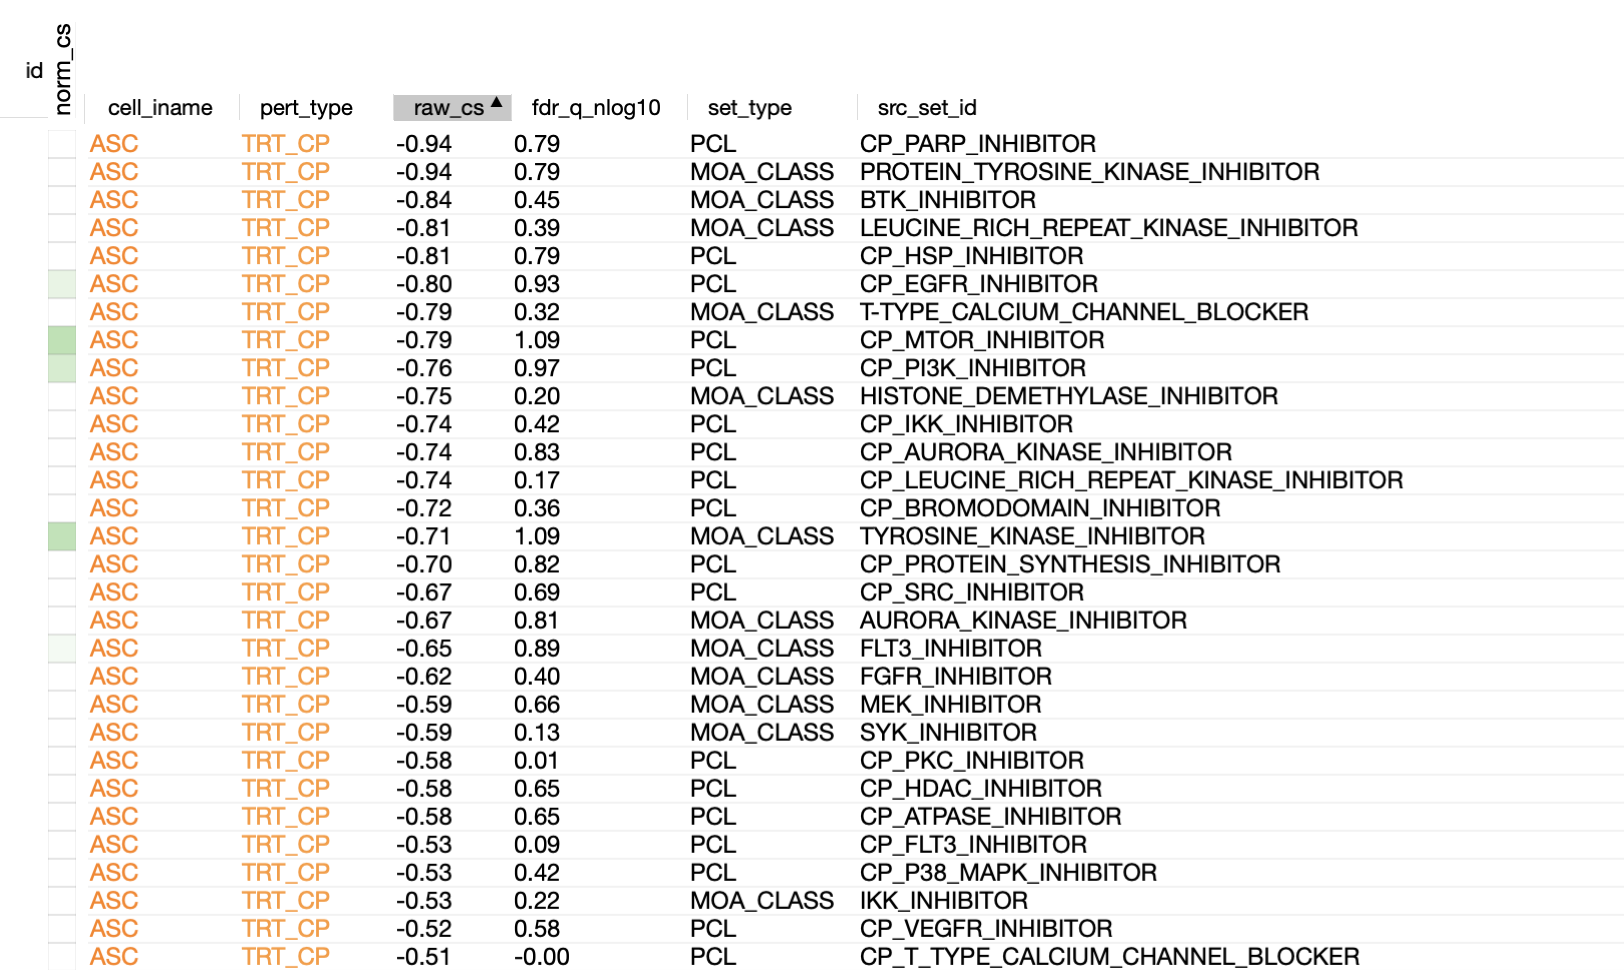
\includegraphics[width=\textwidth]{Figures/Supp_Fig_Adipose_ASC.png} 
\caption{CMAP results using the \textit{adipose} tissue composite 
transcript as an input. Table includes the top 30 results derived
\textit{only from normal adipocytes} (ASC) regardless of significance. 
The results are sorted by the correlation of the query to the input 
with the most negative results at the top.
}
\label{fig:clue_adipose_asc}
\end{figure}

\begin{figure}[ht!]
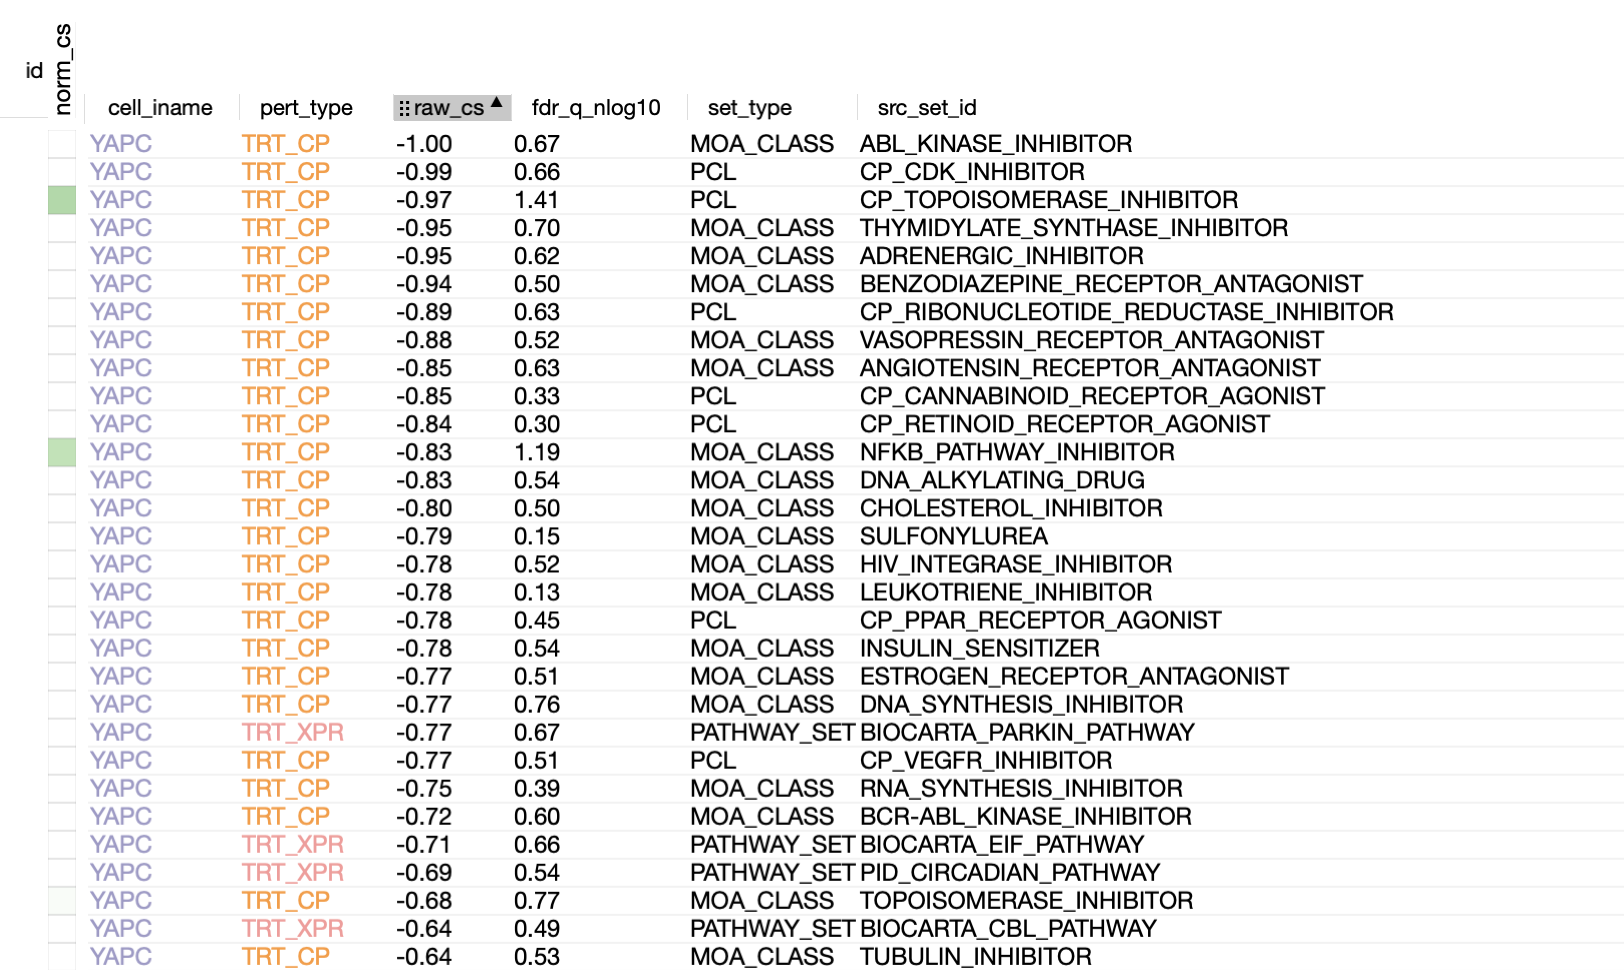
\includegraphics[width=\textwidth]{Figures/Supp_Fig_Islet_YAPC.png} 
\caption{CMAP results using the \textit{pancreatic islet} composite 
transcript as an input. Table includes the top 30 results derived
\textit{only from YAPC cells}, which are derived from pancreatic
carcinoma cells. Results are shown regardless of significance and
are sorted by the correlation of the query to the input 
with the most negative results at the top.
}
\label{fig:clue_islet_yapc}
\end{figure}

\begin{figure}[ht!]
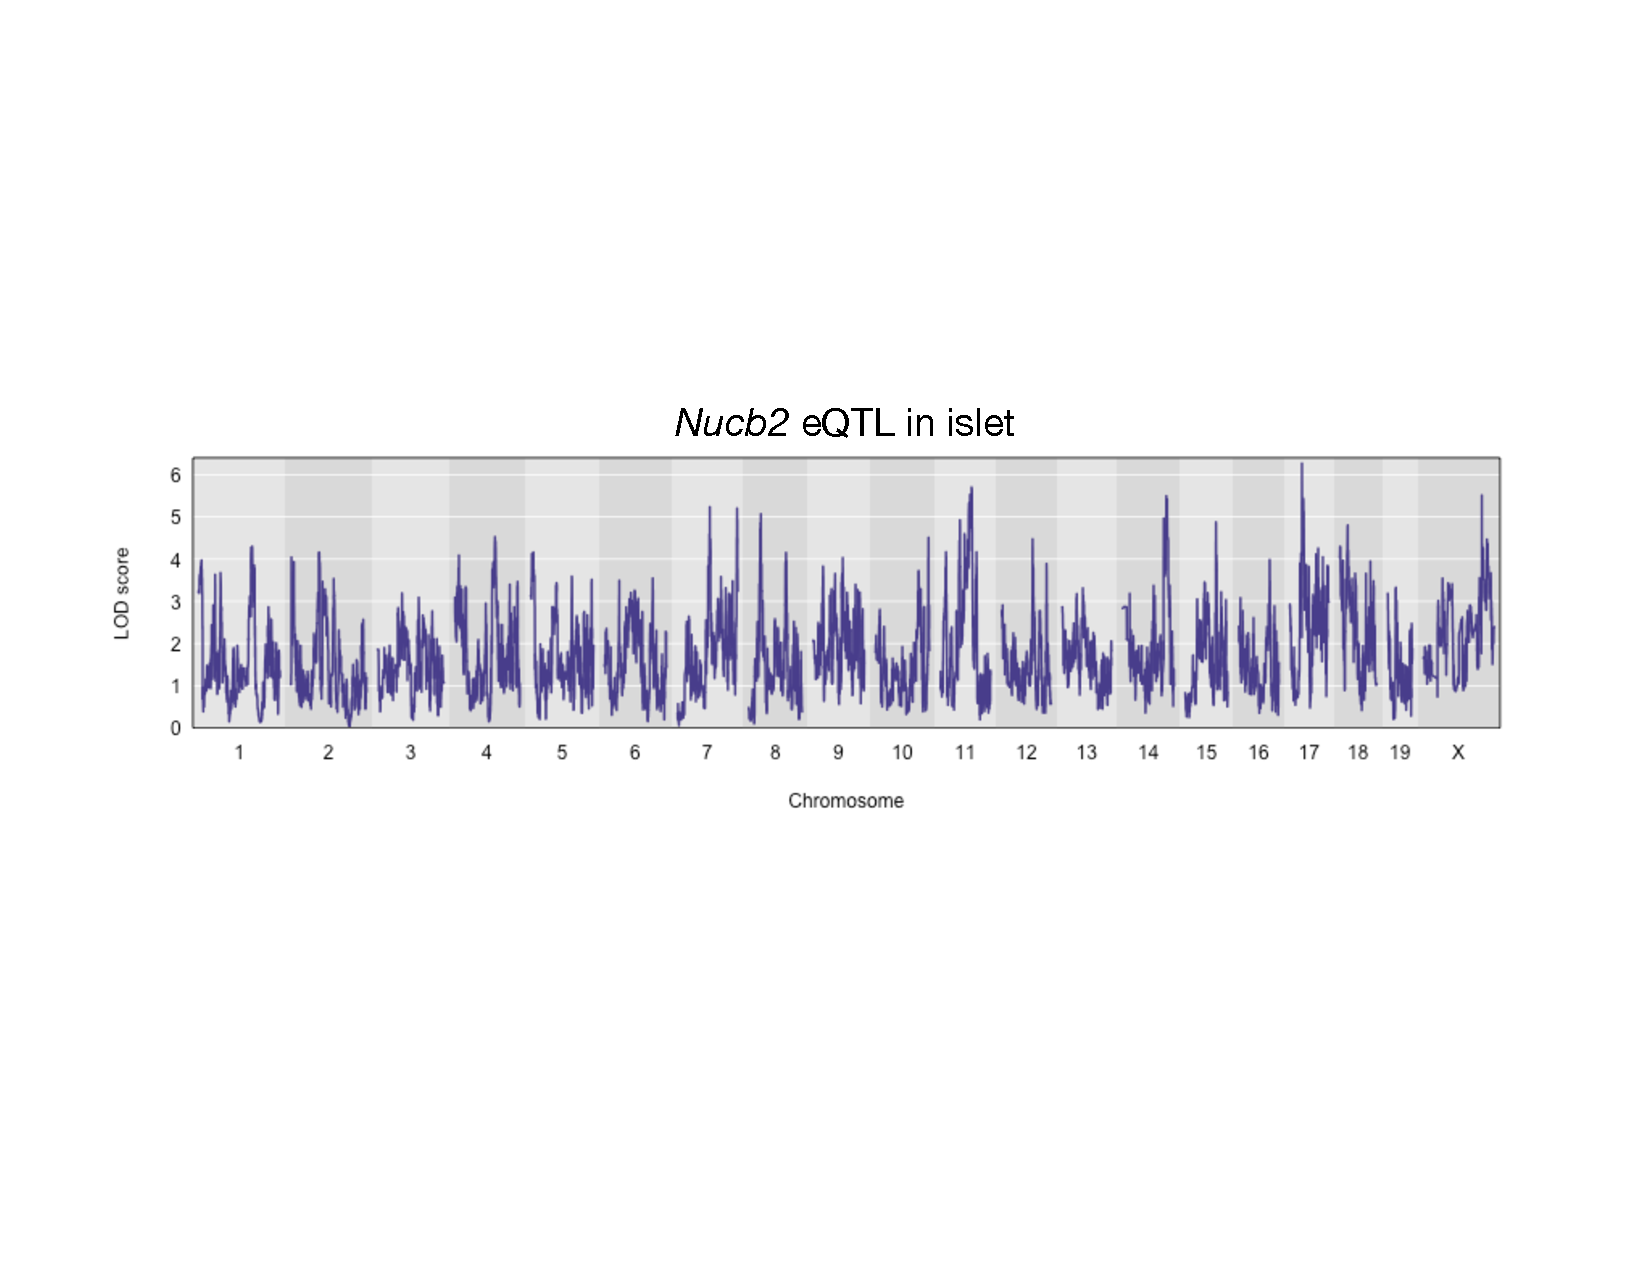
\includegraphics[width=\textwidth]{Figures/Supplemental_FigX_Nucb2_eQTL.pdf} 
\caption{Regulation of \textit{Nucb2} expression in islet. \textit{Nucb2} 
is encoded on mouse chromosome 7 at 116.5 Mb (red line). In islets the 
heritability of \textit{Nucb2} expression levels is 69\% heritable. This 
LOD score trace shows that there is no local eQTL at the position of the
gene, nor any strong distal eQTLs anywhere else in the genome. 
}
\label{fig:Nucb2_eqtl}
\end{figure}

\end{document}
